\chapter{Referencial Teórico}

Para realizar o desenvolvimento da aplicação foi necessário uma fundamentação teórica, apresentando outras literaturas, de forma que a escolha das tecnologias a serem utilizadas fossem guiadas através deste embasamento.
%Neste capítulo será demonstrado a teoria do estudo em questão, apresentando outras literaturas que foram utilizadas para construção do embasamento teórico necessário para a construção desse trabalho.

\section{Extração Automática de Informações em PDF}

Desde sua criação até os dias atuais a utilização de arquivos PDF só cresce, e é o formato mais utilizado para troca de documentos.
Extrair dados através de textos em documentos é um objetivo de interesse de muitos que desejam juntar informações que se encontram isoladas em tais, porém não é uma tarefa simples, principalmente, se tratando de arquivos PDF. A extração automatizada encontra muitas barreiras, de diversas naturezas, e soluções mais genéricas a este problema não são tão comuns (\citeauthor{ajedig2011pdf}, \citeyear{ajedig2011pdf}).

\subsection{PDF - \textit{Portable Document Format}}

Como definido no manual da Adobe Systems (\citeauthor{bienz1993portable}, \citeyear{bienz1993portable}), o PDF é um formato de arquivo para representar um documento de forma que não haja a dependências como fonte, imagens e anexos. O que quer dizer que ele tem a capacidade de reunir todos os recursos necessários para que a visualização do documento não dependa de nenhuma fonte externa.

Com o objetivo de compartilhar documentos digitais, em 1992 a Adobe Systems realizou o lançamento do formato PDF. Em 1993 o formato foi disponibilizado de forma gratuita, o que gerou um grande aumento em sua adoção, mas somente em 2008 ele deixou de ser um formato proprietário e passou a ser um Padrão Aberto, isto significa que qualquer pessoa pode ter acesso a implementação deste formato e não é mais possível ser cobrado royalties pelo uso do mesmo. No mesmo ano foi publicada a ISO 32000-1 (\citeauthor{ISO32000}, \citeyear{ISO32000}) declarando o PDF como um padrão internacional verdadeiramente aberto. A capacidade de gerar um documento fiel a sua criação, e possível de ser visualizado em qualquer dispositivo, que possua um leitor do formato, contribuiu para que ele se tornasse um dos formatos de documento digital mais utilizado no mundo (\cite{adobePDF}).

O PDF é descendente do \textit{PostScript}, uma linguagem de descrição de páginas que inicialmente foi criada para gerar páginas a serem impressas, essa linguagem foi desenvolvida pela \textit{Adobe Systems} e os objetos encontrados no código de arquivos PDF possui sintaxe similar a tal linguagem (\citeauthor{preface2001pdf}, \citeyear{preface2001pdf}).  Como podemos ver na \textbf{Figura \ref{PDF_Structure}}, a estrutura do PDF é dividida em quatro partes: 

\begin{itemize}
    \item Cabeçalho: Contém o número da versão do PDF que foi utilizado para gerar tal documento.
    
    \item Corpo: Aqui está presente todo o conteúdo que pode ser visualizado no documento. Toda informação pertencente ao corpo é dividida em objetos para a informação que será visualizada em cada página. O que engloba texto, imagens, fontes, etc.
    Para fins de otimização os objetos encontrados no corpo não se repetem mesmo estando presente em diferentes páginas.
    
    \item Tabela de Referência Cruzada (\textit{XREF Table}): Essa tabela é responsável por indicar o posicionamento dos objetos no corpo. Desta forma não é necessária a leitura de todo o corpo para que seja encontrado o objeto necessário para compor a visualização.
    
    \item Trailer: Contém a localização do Corpo, da Tabela de Referência Cruzada e o fim do arquivo. O leitor de arquivos PDF irá acessar primeiro o Trailer para saber onde encontrar a tabela e assim carregar os objetos necessários.
\end{itemize}


\begin{figure}
\centering
\captionsetup{justification   = raggedright,
              singlelinecheck = false}
\caption{Detalhamento da estrutura do PDF}\label{PDF_Structure}
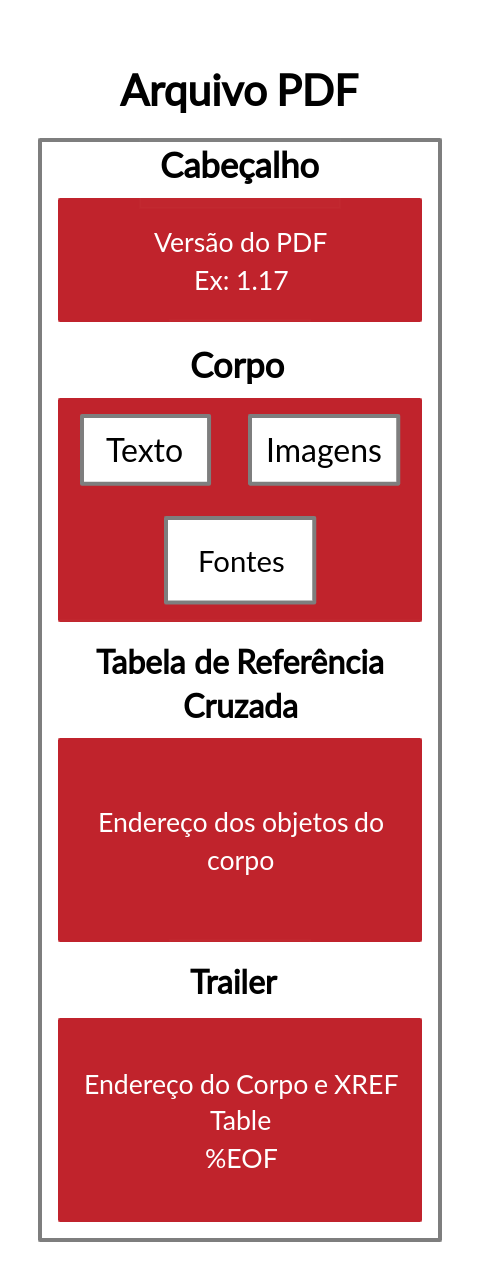
\includegraphics[width=0.3\textwidth]{figs/PDF.png}
\end{figure}

\subsection{Obstáculos na Análise dos Dados}

A extração e análise de dados na área acadêmica é um problema abordado desde a padronização e reconhecimento dos arquivos PDF como um formato universal. O seu crescimento faz com que a análise e extração destes documentos recebam cada vez mais atenção, de diferentes áreas. Como já podem ser encontradas pesquisas que abordam o reconhecimento de fórmulas matemáticas, códigos genéticos, gráficos, entre outras informações. Por ser mais conveniente, são buscadas ferramentas que transformem o arquivo em uma forma intermediária, como por exemplo texto ou HTML, para que seja mais fácil a extração e análise de dados (\citeauthor{ajedig2011pdf}, \citeyear{ajedig2011pdf}).

Com essas abordagens, chegam os desafios, como exemplo, a falta de estrutura padronizada, diferentes formatos dado o software que gerou o arquivo, a incapacidade de renderizar o conteúdo corretamente entre outros. Como foi apresentado no tópico anterior, sabemos que a fonte do PDF não contém as informações de uma forma coerente a leitura humana, e sim blocos que são distribuídos e montados no momento da visualização do arquivo, assim, é necessária realizar uma abordagem na qual as informações buscadas sejam coerentes e não blocos soltos. Outra dificuldade que é muito encontrada está nas diferentes formas que um software pode gerar um arquivo PDF, como no LaTeX, onde certos símbolos matemáticos são desenhados como objetos e no Microsoft Word são utilizados os símbolos Unicode (\citeauthor{sasirekhatext}, \citeyear{sasirekhatext}). A abordagem através do reconhecimento de imagem é muito comum mas enfrenta um grande problema como falsos positivos (\citeauthor{ajedig2011pdf}, \citeyear{ajedig2011pdf}).

Com o objetivo de criar algo mais genérico e reaproveitável para o meio acadêmico, foi pensando em uma forma mais volátil de se realizar a análise dos dados diretamente do PDF montado, e superar as barreiras citadas anteriormente.

\section{Tecnologias}
Como um dos objetivos deste desenvolvimento é criar uma ferramenta que pudesse ser acoplada a outras aplicações e fornecesse a liberdade de ser utilizada em diferentes partes de \textit{front-end}, foi escolhido o formato de API. 

\subsection{API - Interface de Programação de Aplicações}
Uma API é um software intermediário que permite a interação com diferentes aplicações. Ela vai além do que seu nome sugere, e atua principalmente na questão de interface, o grande foco de tal está na forma em que ela se apresenta, isso se tratando de quem a consome, que pode ser tanto para programas quanto para humanos. E se tratando de uma API web, essa interface pode ser acessada em qualquer lugar do mundo. Ela atua recebendo requisições de outra aplicação, então uma rotina correspondente é executada e uma resposta é devolvida a aplicação que realizou a requisição (\citeauthor{designingapioriley}, \citeyear{designingapioriley}).

\begin{enumerate}
  \item REST - Transferência de Estado Representativo
  
  Fielding et al. (\citeyear{fielding2000rest}) propôs em sua tese de doutorado, comparando com estilos arquiteturais já existentes, um estilo para API onde as necessidades de uma aplicação em rede fosse atendidas da melhor forma, e conseguissem que o desenvolvedor seguisse esse padrão sem grandes complicações. Os principais benefícios trazidos pelo REST contam com (\citeauthor{rest2018or}, \citeyear{rest2018or}):
  
  \begin{itemize}
    \item Performance: Resultante de uma comunicação simples e eficiente.
    \item Escalabilidade: Havendo interações simples, é mais prático o crescimento do sistema.
    \item Simplicidade de Interface: Uma interface simples garante uma interação simples e consequentemente traz benefícios como os citados anteriormente.
    \item Manipulação de componentes: Seguindo este estilo há uma separação de responsabilidades, logo um componente não deve depender do outro o que permite que a alteração de um não cause danos a outros.
    \item Portabilidade: Com uma comunicação e Interface simples qualquer API que adote o estilo REST consegue ser consumida por qualquer tipo de tecnologia.
    \item Confiabilidade: Devido a suas restrições, cada requisição é um processo independente o que facilita na recuperação em caso de falhas.
    \item Visibilidade: A Restrição Stateless determina que cada requisição deve ser independente, logo, se forem feitas diversas requisições cada uma deve ter sua resposta e a visibilidade das respostas não precisam ser analisadas.
  \end{itemize}
  
  Fielding et al. (\citeyear{fielding2000rest}) abordou a definição do REST a partir de restrições, elas definem limites e regras para os componentes que compõe o sistema. São seis restrições: 
  
  \begin{enumerate}
    \item Client-Server: É a restrição mais básica, ela garante que a API irá lidar com a comunicação com o banco de dados, gerenciamento de cache, log, etc. Desta forma são separadas as responsabilidades do front-end e do back-end.
    \item Stateless: Como dito anteriormente, esta restrição diz que o cliente pode fazer várias requisições, isso significa que para cada requisição que ele fizer deve ser enviado todas as informações novamente.
    \item Cacheable: Esta restrição não precisa ser aplicados para todos componentes, ela define que a informação de resposta deve ser guardada em cache. No caso de muitas requisições a mesma informação não é necessário ocorrer todo o processo de busca no banco de dados e processar os dados.
    \item Uniform Interface: Tendo uma interface uniforme para todas as requisições o cliente sabe exatamente o formato de resposta que ele deve esperar e é possível ter o mesmo resultado para diferentes plataformas que estiverem consumindo a API.
    \item Layered System: Tendo em mente que que a API está conectada a internet e deve ocorrer um grande tráfego de informação, é aplicado o conceito de camadas para que haja uma simplificação do sistema e uma boa organização dos componentes. Cada camada tem sua responsabilidade, como por exemplo executar a lógica e buscar ou salvar informações.
    \item Code-On-Demand: Única restrição opcional, ela permite que o cliente execute código da lógica do servidor através de um script.
  \end{enumerate}
  
  Estas restrições atuam como paredes invisíveis e conseguem guiar o desenvolvedor. Aplicando estas condições no código é possível obter várias vantagens e construir uma API de ótima performance, coesa e escalável.Quando estas restrições são aplicadas de forma correta no projeto, é utilizada a expressão RESTful para identificar que aquela API está incorporando os limites dado pelo estilo de arquitetura REST.

  \item XML vs JSON
  
  \citeauthor{xml2012} descrevem que o massivo aumento da web trouxe uma grande necessidade de um formato para troca de dados entre diferentes tecnologias. Não havia um formato padronizado de forma que, automaticamente, os dados exportados fossem entendidos ao serem importados em outra aplicação. Com essa necessidade \cite{Sperberg-McQueen:08:EML} junto ao W3C, criaram o XML (\textit{Extended Markup Language}), sendo uma linguagem de marcação, assim como o HTML, mas atendendo a demanda da troca de dados. Atualmente é a forma mais adotada para documentação e registro de dados simples.
  
  Atualmente existem várias alternativas ao XML, sendo as mais famosas JSON e YAML, neste tópico trataremos apenas da comparação com o JSON. O \textit{JavaScript Object Notation} (JSON) é um formato de texto criado para representar um objeto JavaScript, de forma simples, portável e textual (\citeauthor{json2014disponivel}, \citeyear{json2014disponivel}). 
  
  Se tratando uma forma mais compacta, menos verborrágica e com o crescimento do número de aplicações escritas em JavaScript, o JSON se tornou muito popular e vem tomando espaço do XML quando se trata de troca de dados entre plataformas. \citeauthor{xml2012} realizaram uma comparação onde as seguintes vantagens são atribuídas ao JSON.
  
  \begin{itemize}
      \item Velocidade: A análise e leitura de arquivos XML tendem a ser lentas, devido a sua verborragia, enquanto o JSON entrega os dados de forma simples e direta.
      
     \item Serialização e Desserialização: Normalmente é encontrada uma única forma, e já presente no JavaScript, para a transformação dos dados de JSON para bytes, e vise-versa.
     
     \item Conciso: O JSON utiliza a técnica de chave-valor, enquanto o XML utiliza tags, o que dificulta a visualização e aumento o tamanho do arquivo.
     
     \item Bibliotecas de fácil utilização: Atualmente é possível encontrar bibliotecas, para a maioria das linguagens, que tornam a utilização do JSON muito orgânica, enquanto a utilização do XML é algo mais complicado.
  \end{itemize}
  
  Dado as vantagens, e a escolha do Node.js, que será melhor abordada no próximo tópico, foi decidido que todos os dados na aplicação serão trabalhados no formato JSON.
  
  \item \textit{Middleware}
  
  
  
\subsection{Node.JS}

Node é a forma de utilizar JavaScript em um servidor. A implementação do Node tem base no interpretador JavaScript desenvolvido pela Google, o V8, este interpretador é implementado em C e C++, e se concentra em extrair a melhor performance utilizando menos memória (\citeauthor{tilkov2010node}, \citeyear{tilkov2010node}). 

Motivado a criar uma comunicação simples entre o servidor e a página web, Ryan Dahl criou o Node.js em 2009 e foi um sucesso imediato. Fundamentado em ser Event Driven, o que quer dizer que há sempre um core escutando por todos os eventos, e chamando as devidas funções quando tais eventos são acionados; somado com o JavaScript foi obtido um web server rápido e acessível a toda comunidade web que já tinha familiaridade com a linguagem, o que foi essencial para que o Node fosse tão amplamente adotado (\citeauthor{shah2017node}, \citeyear{shah2017node}).

A introdução do Node trouxe características de outras linguagens que não existem no JavaScript no navegador, como a manipulação do sistema de arquivos, acesso a um banco de dados e a criação de um cliente HTTP, o que faz possível a criação de um web server  (\citeauthor{mead2018learning}, \citeyear{mead2018learning}). Pela familiaridade de grande parte dos desenvolvedores web com a linguagem JavaScript e a crescente onde de separação de Front-End e Back-End, a criação de API's utilizando o Node.JS se tornou muito popular e atualmente, boa parte das ferramentas encontradas para atingir os objetivos deste trabalho podem ser encontradas como bibliotecas de tal.

\begin{enumerate}
    \item NPM - \textit{Node Package Manager}
    No mesmo ano de lançamento do Node.JS foi lançado o \textit{Node Package Manager} (NPM), que atua como um gerenciador e distribuidor de pacotes para projetos, e conta com uma interface por linha de comando que auxilia na criação e manejo de tais. 
    Atualmente o NPM é o maior registrador de software do mundo, devido a sua facilidade e a imensa comunidade dos usuários. 
    Em poucos segundos é possível submeter um pacote ao NPM e assim com a visibilidade e apoio da comunidade este pacote é mantido e utilizado livremente por desenvolvedores ao redor do mundo. Muitas tarefas específicas e morosas são evitadas através da utilização de algum pacote que já contém determinada solução para tal tarefa.
    Uma importante tarefa que o mesmo executa é o controle de versão de dependências, isto é, um pacote pode utilizar determinada versão de outro, e através de um arquivo chamado \textit{lockfile} é obtida determinada versão da dependência de forma que o pacote não encontre problemas de outras versões da dependência. A utilização do NPM em projetos Node é algo indispensável e de grande utilidade. Desta forma, este foi utilizado para o controle de bibliotecas e organização do projeto (\citeauthor{npm}, \citeyear{npm}).

\end{enumerate}

\subsection{NoSQL}

Estabelecido que o sistema terá como base uma API em Node.JS, foi necessário escolher um banco de dados. Pensando na melhor integração com o Node.JS, a possibilidade de escalar para uma massiva quantidade de dados e a compatibilidade com chave-valor proveniente dos objetos JSON; foi feita uma análise dos bancos NoSQL.

O NoSQL é uma categoria de banco de dados que surgiu com o objetivo de atender aos requisitos do gerenciamento de grande volume de dados, sem estrutura definida e que necessitam ser disponibilizados rapidamente e preparados para crescer ainda mais. Esta categoria traz algumas características como: (\citeauthor{loscio2011nosql}, \citeyear{loscio2011nosql}).

\begin{itemize}
    \item Evitamento de Complexidade desnecessária.
    \item Alta Taxa de Transferência: A maioria dos bancos não relacionais conseguem ter uma boa vantagem na taxa de transferência quando comparados aos relacionais.
    \item Escalabilidade Horizontal.
    \item Esquema Flexível ou Ausência de Esquema: A ausência ou flexibilidade de esquema trás vantagens como a alta escalabilidade e a oportunidade de mudar ou adicionar campos inesperados. Há a desvantagem da falta de garantia de integridade dos dados.
    \item Simples Acesso aos Dados: Com o foco em velocidade é essencial que a entrega de dados ao sistema seja feita de forma simples e enxuta, o modelo NoSQL oferece os dados como interface e facilita o acesso e utilização de tal.
    \item Modelo Chave-Valor: O modelo simples torna prático o armazenamento de dados, principalmente quando se trata de algo que não necessita se relacionar com outros valores e independe do tamanho do valor.
\end{itemize}
  
\section{Estado da Arte}  

Se tratando de outros programas que em sua essência realizam a análise extração de dados foram encontradas boas alternativas, mas nenhuma que contemplasse todos os objetivos que foram postos aqui. A seguir serão apresentadas essas alternativas e definido porque ela não se encaixa no objetivo deste projeto.

\begin{itemize}
    \item \cite{pdft}, \cite{fpdfc} e \cite{tabula} São boas alternativas, grátis mas que realizam apenas a extração de dados tabulares e geram arquivos \textit{.csv}. Não satisfazendo os quesitos de ser genérico e ter a capacidade de se acoplar a outra aplicação.
    
    \item \cite{lapdf} é uma alternativa desenvolvida por biomédicos que buscavam extrair dados de artigos, ela ainda está em desenvolvimento, porém o foco dela é a extração de dados somente de artigos. Assim, ela está engessada ao layout de artigos e não funciona com outros tipos de arquivo. Apresenta as mesmas incapacidades das alternativas anteriores, quanto aos objetivos deste projeto.
    
    \item \cite{epdf} é uma alternativa online e grátis que realiza a conversão do PDF em arquivos de texto e imagens. Em testes feitos neste site, foi notado que a extração de texto é feita em blocos quebrados que nem sempre estão na ordem correta de leitura. Não torna possível a utilização em outras aplicações e não possibilita a seleção de quais dados serão extraídos.
    
    \item \cite{dparser} apesar de ser uma alternativa paga, pelo que foi apresentado realiza a extração dos dados dada as coordenadas e página, resultando em um arquivo de texto com os dados extraídos. 
    
    \item \cite{ipdf} Uma ótima alternativa que pode ser utilizada com aplicações em Java e C++, possui uma API e uma interface amigável caso necessário, e diversos modos de configuração para que se atinja a extração do dado necessário. Porém é uma alternativa paga.
    
\end{itemize}

\end{enumerate}